\documentclass[border=10pt]{standalone}
\usepackage{tikz}
\usepackage{amsmath}
\usetikzlibrary{arrows.meta, shapes, calc}

\begin{document}
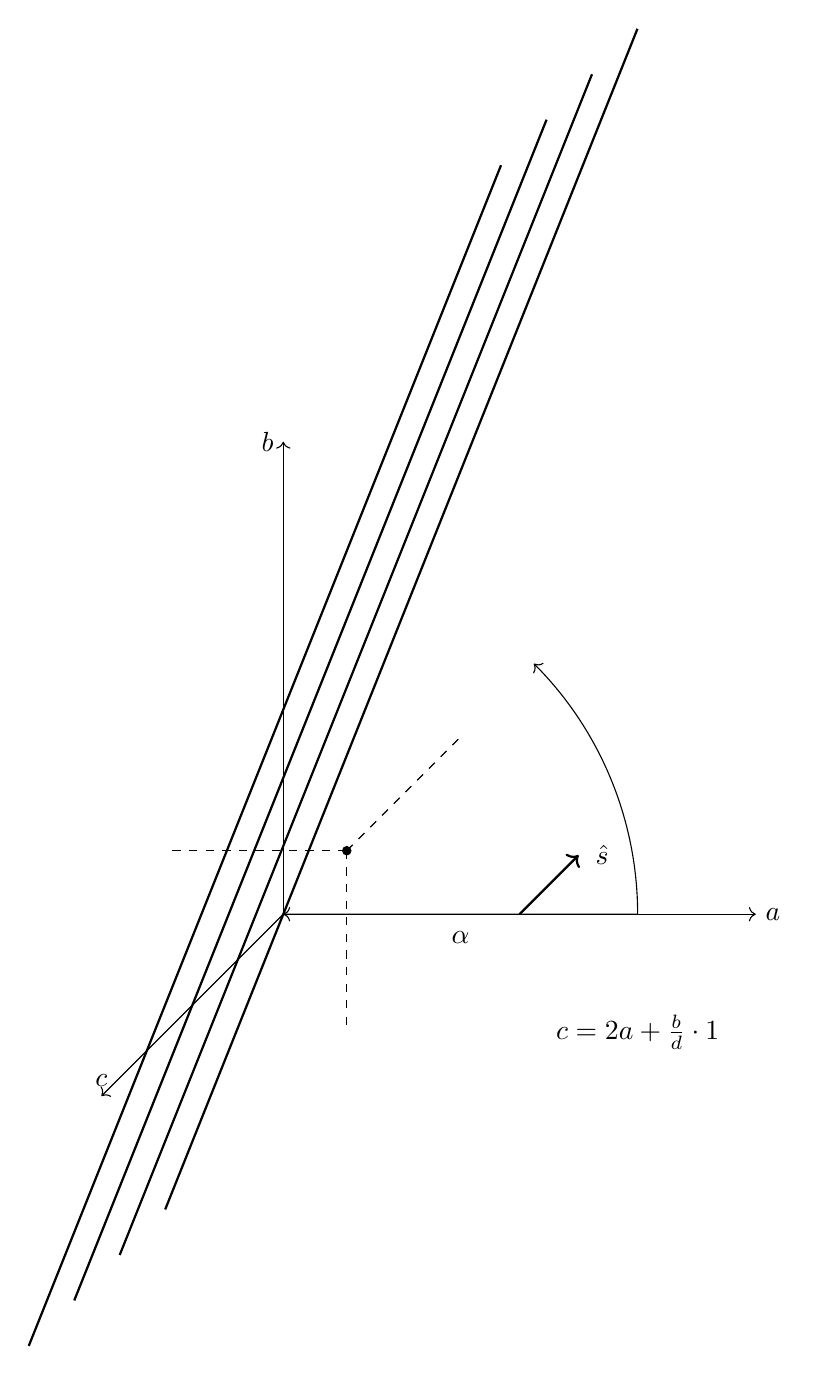
\begin{tikzpicture}[scale=1.5]

  % Axes
  \draw[->] (0,0,0) -- (0,0,4) node[above] {$c$};
  \draw[->] (0,0,0) -- (4,0,0) node[right] {$a$};
  \draw[->] (0,0,0) -- (0,4,0) node[left] {$b$};

  % Plane
  \draw[thick, domain=-1:3, samples=100] plot (\x, {2*\x + 1/2*\x}, 0);
  \draw[thick, domain=-1:3, samples=100] plot (\x, {2*\x + 1/2*\x}, 1);
  \draw[thick, domain=-1:3, samples=100] plot (\x, {2*\x + 1/2*\x}, 2);
  \draw[thick, domain=-1:3, samples=100] plot (\x, {2*\x + 1/2*\x}, 3);

  % Point
  \filldraw[black] (1.5, 1.5, 2.5) circle (1pt);

  % Dashed lines for projection
  \draw[dashed] (1.5, 1.5, 2.5) -- (1.5, 1.5, 0);
  \draw[dashed] (1.5, 1.5, 2.5) -- (1.5, 0, 2.5);
  \draw[dashed] (1.5, 1.5, 2.5) -- (0, 1.5, 2.5);

  % Angle alpha
  \draw[<->] (0,0,0) -- (3,0,0) arc (0:45:3);
  \node at (1.5, -0.2) {$\alpha$};

  % Vector ŝ
  \draw[->, thick] (2,0,0) -- (2.5, 0.5, 0);
  \node at (2.7, 0.5) {$\hat{s}$};

  % Equation
  \node at (3, -1) {$c = 2a + \frac{b}{d} \cdot 1$};

\end{tikzpicture}
\end{document}